% -*- root: ./report.tex -*-
\chapter{Results \& Discussion}\label{chap:results}
		In this chapter, we show how some properties of the system change by the introduction of a zigzag geometry.
		Additionally, we attempt to isolate the mechanism behind the improved properties by estimating the gap size through the quasiclassical model introduced in chapter \ref{chap:methods}.
		
	\comment{Introduction of a zigzag opens up the gap, creates a more stable topological phase diagram, and decreases coherence length of Majoranas}
	\section{Increased isolation and stability of the Majorana state}

		\comment{We see that the introduction of a zigzag leads to a reduction of the gap}
		\subsection{Gap/bandstructure as a function of zigzagginess}

			\begin{figure}[!htb]
			\centering
			\includegraphics[width=0.55\columnwidth]{figures/bandstructures}
			\caption{Figure of the bandstuctures corresponding to the system in Fig.~\ref{fig:zigzag_methods}.
			Blue lines correspond to $\phi=0$, $B=0$, red lines to $\phi=\pi$, $B = 1$.
			Thre three subplots are for different amplitudes of zigzag: (a) $z_y=0$, (b) $z_y=\frac{W}{4}$, and (c) $z_y=\frac{W}{2}$, where $W=200$\si{\nm} is the junction width.
			We observe that once there are no more straight trajectories inside the junction (when $z_y=\frac{W}{2}$) the spectrum becomes most insensitive to the momentum $k_x$.
			The value of the remaining parameters are, $\alpha=20$ \si{\milli \eV \nm}, $g=26$, $\meff=0.02$\si{\electronmass}, $\mu=20$ \si{\milli \eV}, $\Delta=1$ \si{\milli \eV}.
			\label{fig:bandstuctures}}
			\end{figure}

			\comment{We calculate the bandstructure for varying amount of zigzag.}
			We implement a tight-binding version of the model described in section \ref{sec:physical_picture}.
			In figure~\ref{fig:bandstuctures}, the bandstructure for saw toothed zigzag systems [Fig.~\ref{fig:zigzag_methods}] with varying amplitude is displayed.
			Because the zigzag has to be modeled using a supercell, we see a folded bandstructure.
			For comparison's sake, we take the same cell size for the ribbon structure so the bandstructure is folded in the same way.

			\comment{The band structures show that modulation of the geometry increases the gap by an order of magnitude, as well as reduce the group velocity.}
			The introduction of a zigzag has a striking effect: the bands flatten out, and more importantly, the gap size is increased more than an order of magnitude.
			This happens because the modes where the gap is the smallest when the momentum is almost completely focused along the strip ($k_x=k_F$), are cut off in a zigzag geometry.
			There is also a significant reduction of the group velocity where in Fig.~\ref{fig:bandstuctures} (c) the bands are almost completely flat.
			The size of the gap, together with the velocity, directly relate to the Majorana coherence length (Eq.~\eqref{eq:majorana_coherence_length}), which will be discussed in the following section.

			\comment{The introduction of an SN interface at many angles also increases performance.}
			Finally, in the presence of normal reflection, due to the availability of NS interfaces at a wide range of slopes, a zigzag system has an increased effective transmission.
			In a zigzag system, the normally reflected part of a wavefunction will eventually intersect a surface with which it is nearly perpendicular to.
			The transparency of the NS interface is thus improved for non-transversal modes.

		\comment{Introduction of a zigzag leads to localization of the Majoranas}
		\subsection{Majorana decay length}

			\comment{We calculate the lowest eigenfunction and plot the density.}
			Using the tight-binding package Kwant~\cite{groth_kwant:_2014}, we model a finite system to compute the Majorana wave function density for different geometries; ribbon, zigzag, parallel curve, and vertically offset sinusoids.
			In figure~\ref{fig:wavefunctions} the wavefunctions superimposed upon their respective geometry are displayed including the corresponding Majorana energies $E_M$, as well as $E_1$: the energies corresponding to the next lowest state.

			\begin{figure}[!htb]
			\centering
			\includegraphics[width=0.55\columnwidth]{figures/wavefunctions}
			\caption{Wavefunctions for different sizes and geometries.
			With (a) a straight system, (b) a zigzag system, (c) a system where the normal region is defined by lines parallel to a sinusoid, and (d) a system with vertically offset sinusoids.
			Inside the figure, we indicate the Majorana length (or coherence length) $\xi$ and the topological energy gap $E_\textrm{gap}$.
			We observe that $\xi$ for (a) is orders of magnitude longer and $E_\textrm{gap} = E_\textrm{1} - E_M$ orders of magnitude smaller than for (b, c, d), meaning that the details of the geometry do not matter.
			\label{fig:wavefunctions}}
			\end{figure}

			\comment{In a straight system, the Majoranas are very poorly localized.}
			For the ribbon system [Fig.~\ref{fig:wavefunction}(a)], we see that the decay of the density is long compared to the system size.
			We see that the wavefunction extends to the center of the system, not showing the delocalization sought after.
			Apart from the density, as discussed in chapter \ref{chap:theory}, overlap of Majoranas leads to a non-zero energy of the state.
			Taking this into consideration, we see that the energy of the Majorana state in the straight system is only barely below the next lowest lying eigenstate: the Majoranas are very poorly localized and topological protection against perturbations is minimal.
			
			\comment{In a zigzag geometry Majoranas are localized within one segment of zigzag.}
			All of the zigzag type geometries show a greatly reduced coherence length.
			The delocalized nature of the wavefunctions is clearly visible through the density plots.
			Quantitatively, the improvement in the localization of the Majoranas is also distinctly apparent: the energies of the Majorana states are three orders of magnitude lower than the energy of the second lowest-lying wavefunctions.
			As mentioned in the previous section, this can be attributed to the way the gap and velocity factor into the Majorana coherence length.

			\comment{We also confirm that the specific shape does not matter.}
			The shape of the wavefunctions does not change significantly depending on the details of the shape.
			The sharp corners of the sawtooth versus the smooth shape of the snakelike system do not have a great impact on the shape of the wavefunction.


		\comment{Zigzag Majoranas have a cleaner phase diagram due to the reduction in symmetry class}
		\subsection{Phase diagram}

			\comment{We calculate the topological phase diagram using the gap size.}
			Due to the size of the system, we cannot use full spectrum methods (the Pfaffian in this case) to compute the topological invariant of our system.
			Instead, we calculate the gap by finding the absolute minimum of the spectrum $E_\textrm{gap}=\min{|E(k)|}$.
			Noting the gap closings, and that we know the topological phase for the non-zigzag system (e.g. for magnetic field vs. phase difference it is diamond shaped: Fig.~\ref{fig:pientka_phase_diagram}), we can infer the topology of the system with zigzag modulation.
			In figure ~\ref{fig:phasediagrams}, we plot the energy gap as a function of magnetic field, chemical potential, and the superconducting phase difference for both a straight system [(a) and (b)] and a zigzag system [(c) and (d)].

			\begin{figure}[!htb]
			\centering
			\includegraphics[width=0.75\columnwidth]{figures/phasediagrams}
			\caption{Phase diagrams of a straight system (a), (b) and zigzag system (c), (d), where (a), (c) are $E(\mu, B)$ and (b), (d) are $E(\phi, B)$.
			We use a generalized eigenvalue problem to find all phase boundaries at once and find the minimal energy gap by finding the minimum in the spectrum: $\min{E(k)}$.
			\label{fig:phasediagrams}}
			\end{figure}

			\comment{The phase diagram does not change much, except we see a cleaner spectrum as a result of the D class symmetry. }
			Similar to what is described by Pientka et. al~\cite{pientka2017topological} (see Fig.~\ref{fig:pientka_phase_diagram}), we see that the straight geometry, as a function of superconducting phase difference and Zeeman field (b), has a diamond-shaped phase diagram.
			The additional gap closings visible within the diamond are due to the system belonging to the BDI symmetry class and cause the region of interest, where there is a single pair of Majoranas, to be relatively small.
			
			For the zigzag system, the magnitude of the gap is significantly improved, as expected.
			The diamond-like shape of the phase-Zeeman plot is retained, and there is no significant change in its size either.
			We expect a cleaner phase diagram due to the system belonging to the D symmetry class, which is partially reflected in the diagram: there is a large and stable (no gap closings) central region, but near 0 and 2$\pi$ phase difference, in the corner of the diamond, we see a chaotic collection of gap closings.
			We are unsure of the nature of these gap closings, but they can perhaps be attributed to the symmetry breaking being relatively weak.



	\section{Finding the mechanism responsible for the increased gap}
		\comment{We compare different techniques to calculate the band structure of a straight system.}
		We verify the validity of the analytic model described in the Methods, to compute the bandstructure of a straight system in a tilted magnetic field.
		In Fig.\ref{fig:spectrum_calculation_comparison}, we compare the analytical model with band structures obtained using three different methods, implemented in Kwant.
		To show that the model has been correctly implemented, we compute the Kwant scattering matrix of the identical model used in the analytics and substitute it into the bound state condition\eqref{eq:bound_state_condition_sjl} (labeled Kwant without SOI SJL).
		To show the validity of neglecting spin-orbit in the transverse direction, we also compute the scattering matrix including the additional term and again use the bound state condition to obtain the spectrum (labeled Kwant with SOI SJL).
		We also perform the fully accurate calculation of the spectrum by simply computing the bandstructure of the corresponding Kwant system (labeled Full ribbon Kwant system): this result serves as the benchmark for the other techniques.

		\subsection{Verification of analytical estimate}
			\begin{figure}[!htb]
			\centering
			\includegraphics[width=0.95\columnwidth]{figures/spectrum_calculation_comparison}
			\caption{Andreev Bound State spectrum of a SNS junction with a tilted in-plane magnetic field, computed using four different methods.}.
			\label{fig:spectrum_calculation_comparison}
			\end{figure}
		
			All three of the scattering matrix approaches agree almost perfectly with each other.
			We must note that ignoring spin-orbit coupling in the transverse direction is only valid if the spin-orbit length is sufficiently small compared to the width of the system.
			What is also clear from the plot is that the domain of the scattering matrix methods is limited.
			This is a result of the zero energy approximation used to compute the momenta in the short junction limit: this assumption yields no solutions beyond the Fermi surface.

			When comparing the scattering matrix approach to the full bandstructure calculation, we see that it holds only approximately: the shape of the bands is similar, but the magnitude differs significantly.
			We attribute this to the loose compliance with the short junction limit: one needs both a long superconducting coherence length, as well as the energies in the spectrum to be near zero.
			As we find the accuracy of the analytical spectrum to be relatively weak, we continue estimation of the gap in a zigzag system using the spectrum calculated with the full Kwant system.

		\subsection{Estimation of the gap through momentum cutoff}
			As explained in the Methods chapter, we estimate the topological gap using a quasiclassical estimate.
			We keep the ratio $4\dfrac{z_x}{z_y}$ constant and compute the gap as a function of $z_y$.
			In Figure \ref{fig:quasiclassical_approximation}, the result is shown, comparing numerical gap calculations of the full zigzag system (full lines), with the result of the quasiclassical estimation.
			Note that the quasi-classics are only valid once the zigzag cuts off all trajectories which extend infinitely.
			Also important to note is that for the quasiclassical estimate, we set the longest trajectory to be the trajectory that does not include the corners, as depicted in Fig.~\ref{fig:longest_trajectory_wo_corners}

			\begin{figure}
			\centering
			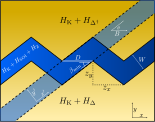
\includegraphics[width=0.45\columnwidth]{images/longest_trajectory_wo_corners}
			\caption{Diagram depicting quasiclassical estimate of a zigzag system, but now with the longest trajectory chosen to avoid the corners of the zigzag.}
			\label{fig:quasiclassical_approximation}
			\end{figure}

			\begin{figure}[!htb]
			\centering
			\includegraphics[width=0.95\columnwidth]{figures/z_y_vs_E_gap}
			\caption{Comparison of the topological gap computed using a full zigzag system implemented in Kwant with the quasiclassical estimate.
			The ratio $4\dfrac{z_x}{z_y}$ is kept constant at three different values, and the gap is calculated for varying $z_y$.
			The full lines represent  the numerical gap calculations of the full zigzag system, the dashed lines represent the quasiclassical estimation.}
			\label{fig:quasiclassical_approximation}
			\end{figure}

			We would expect that the maximum gap improvement would occur near where the zigzag amplitude $z_y$ is large enough to cut off any angle in the system.
			This point is different for the three ratios but can be identified by where the gap is largest for the quasiclassical estimate (dashed lines).
			Increasing $z_y$ further would only allow longer trajectories, which would seem extra undesirable due to the magnetic field not being aligned with the diagonal sections.
			
			Considering the lines corresponding to the full zigzag systems, we see that, for the lower ratios (and thus steeper slopes), the optimal value lies far beyond the cutoff point.
			This is unexpected, and it weakens the validity of the idea that the gap is mostly determined by the length of the trajectories.
			A possible explanation is that for lower ratios, the length of the diagonal sections is smaller, and it is easier for the wavefunction to tunnel through the superconductor.
			In any case, this phenomenon requires additional explanation.

			The quasiclassical estimate, indicated by the dashed lines, seems to consistently underestimate the gap.
			We also see that the gap declines monotonically with respect to the zigzag amplitude, which is by design: increasing the zigzag amplitude corresponds to increasing the domain of permitted trajectories, and thus the minimum can only decrease.
			Even so, we see that the decline of the gap with respect to $z_y$ is much quicker than with an actual zigzag.
			A possible reason that the quasiclassical model sketches a darker picture than full zigzag, is due to the fact that in that model, long trajectories also correspond to grazing angles of incidence at the NS interface.

			We conclude that the proposed model to estimate the gap does not capture the physics of the zigzag very well: the model merely gives a lower bound for the topological gap.
